\documentclass[twoside]{book}

% Packages required by doxygen
\usepackage{fixltx2e}
\usepackage{calc}
\usepackage{doxygen}
\usepackage[export]{adjustbox} % also loads graphicx
\usepackage{graphicx}
\usepackage[utf8]{inputenc}
\usepackage{makeidx}
\usepackage{multicol}
\usepackage{multirow}
\PassOptionsToPackage{warn}{textcomp}
\usepackage{textcomp}
\usepackage[nointegrals]{wasysym}
\usepackage[table]{xcolor}

% Font selection
\usepackage[T1]{fontenc}
\usepackage[scaled=.90]{helvet}
\usepackage{courier}
\usepackage{amssymb}
\usepackage{sectsty}
\renewcommand{\familydefault}{\sfdefault}
\allsectionsfont{%
  \fontseries{bc}\selectfont%
  \color{darkgray}%
}
\renewcommand{\DoxyLabelFont}{%
  \fontseries{bc}\selectfont%
  \color{darkgray}%
}
\newcommand{\+}{\discretionary{\mbox{\scriptsize$\hookleftarrow$}}{}{}}

% Page & text layout
\usepackage{geometry}
\geometry{%
  a4paper,%
  top=2.5cm,%
  bottom=2.5cm,%
  left=2.5cm,%
  right=2.5cm%
}
\tolerance=750
\hfuzz=15pt
\hbadness=750
\setlength{\emergencystretch}{15pt}
\setlength{\parindent}{0cm}
\setlength{\parskip}{3ex plus 2ex minus 2ex}
\makeatletter
\renewcommand{\paragraph}{%
  \@startsection{paragraph}{4}{0ex}{-1.0ex}{1.0ex}{%
    \normalfont\normalsize\bfseries\SS@parafont%
  }%
}
\renewcommand{\subparagraph}{%
  \@startsection{subparagraph}{5}{0ex}{-1.0ex}{1.0ex}{%
    \normalfont\normalsize\bfseries\SS@subparafont%
  }%
}
\makeatother

% Headers & footers
\usepackage{fancyhdr}
\pagestyle{fancyplain}
\fancyhead[LE]{\fancyplain{}{\bfseries\thepage}}
\fancyhead[CE]{\fancyplain{}{}}
\fancyhead[RE]{\fancyplain{}{\bfseries\leftmark}}
\fancyhead[LO]{\fancyplain{}{\bfseries\rightmark}}
\fancyhead[CO]{\fancyplain{}{}}
\fancyhead[RO]{\fancyplain{}{\bfseries\thepage}}
\fancyfoot[LE]{\fancyplain{}{}}
\fancyfoot[CE]{\fancyplain{}{}}
\fancyfoot[RE]{\fancyplain{}{\bfseries\scriptsize Generated by Doxygen }}
\fancyfoot[LO]{\fancyplain{}{\bfseries\scriptsize Generated by Doxygen }}
\fancyfoot[CO]{\fancyplain{}{}}
\fancyfoot[RO]{\fancyplain{}{}}
\renewcommand{\footrulewidth}{0.4pt}
\renewcommand{\chaptermark}[1]{%
  \markboth{#1}{}%
}
\renewcommand{\sectionmark}[1]{%
  \markright{\thesection\ #1}%
}

% Indices & bibliography
\usepackage{natbib}
\usepackage[titles]{tocloft}
\setcounter{tocdepth}{3}
\setcounter{secnumdepth}{5}
\makeindex

% Hyperlinks (required, but should be loaded last)
\usepackage{ifpdf}
\ifpdf
  \usepackage[pdftex,pagebackref=true]{hyperref}
\else
  \usepackage[ps2pdf,pagebackref=true]{hyperref}
\fi
\hypersetup{%
  colorlinks=true,%
  linkcolor=blue,%
  citecolor=blue,%
  unicode%
}

% Custom commands
\newcommand{\clearemptydoublepage}{%
  \newpage{\pagestyle{empty}\cleardoublepage}%
}

\usepackage{caption}
\captionsetup{labelsep=space,justification=centering,font={bf},singlelinecheck=off,skip=4pt,position=top}

%===== C O N T E N T S =====

\begin{document}

% Titlepage & ToC
\hypersetup{pageanchor=false,
             bookmarksnumbered=true,
             pdfencoding=unicode
            }
\pagenumbering{alph}
\begin{titlepage}
\vspace*{7cm}
\begin{center}%
{\Large Interworking Interface }\\
\vspace*{1cm}
{\large Generated by Doxygen 1.8.14}\\
\end{center}
\end{titlepage}
\clearemptydoublepage
\pagenumbering{roman}
\tableofcontents
\clearemptydoublepage
\pagenumbering{arabic}
\hypersetup{pageanchor=true}

%--- Begin generated contents ---
\chapter{R\+E\+A\+D\+ME}
\label{md_README}
\Hypertarget{md_README}
\href{https://api.travis-ci.org/symbiote-h2020/InterworkingInterface}{\tt } \href{https://codecov.io/github/symbiote-h2020/InterworkingInterface}{\tt }

\section*{Interworking\+Interface}
\chapter{Hierarchical Index}
\section{Class Hierarchy}
This inheritance list is sorted roughly, but not completely, alphabetically\+:\begin{DoxyCompactList}
\item \contentsline{section}{eu.\+h2020.\+symbiote.\+controller.\+Interworking\+Interface\+Controller}{\pageref{classeu_1_1h2020_1_1symbiote_1_1controller_1_1InterworkingInterfaceController}}{}
\item \contentsline{section}{eu.\+h2020.\+symbiote.\+controller.\+Rap\+Rest\+Controller}{\pageref{classeu_1_1h2020_1_1symbiote_1_1controller_1_1RapRestController}}{}
\item \contentsline{section}{eu.\+h2020.\+symbiote.\+rpcserver.\+Registration\+Handler\+R\+P\+C\+Server}{\pageref{classeu_1_1h2020_1_1symbiote_1_1rpcserver_1_1RegistrationHandlerRPCServer}}{}
\item Async\+Configurer\+Support\begin{DoxyCompactList}
\item \contentsline{section}{eu.\+h2020.\+symbiote.\+Interworking\+Interface\+Application}{\pageref{classeu_1_1h2020_1_1symbiote_1_1InterworkingInterfaceApplication}}{}
\end{DoxyCompactList}
\item Listenable\+Future\+Callback\begin{DoxyCompactList}
\item \contentsline{section}{eu.\+h2020.\+symbiote.\+controller.\+Rap\+Rest\+Callback$<$ T $>$}{\pageref{classeu_1_1h2020_1_1symbiote_1_1controller_1_1RapRestCallback}}{}
\item \contentsline{section}{eu.\+h2020.\+symbiote.\+rpcserver.\+Rest\+A\+P\+I\+Callback$<$ T $>$}{\pageref{classeu_1_1h2020_1_1symbiote_1_1rpcserver_1_1RestAPICallback}}{}
\end{DoxyCompactList}
\end{DoxyCompactList}

\chapter{Class Index}
\section{Class List}
Here are the classes, structs, unions and interfaces with brief descriptions\+:\begin{DoxyCompactList}
\item\contentsline{section}{\hyperlink{classeu_1_1h2020_1_1symbiote_1_1InterworkingInterfaceApplication}{eu.\+h2020.\+symbiote.\+Interworking\+Interface\+Application} }{\pageref{classeu_1_1h2020_1_1symbiote_1_1InterworkingInterfaceApplication}}{}
\item\contentsline{section}{\hyperlink{classeu_1_1h2020_1_1symbiote_1_1controller_1_1InterworkingInterfaceController}{eu.\+h2020.\+symbiote.\+controller.\+Interworking\+Interface\+Controller} }{\pageref{classeu_1_1h2020_1_1symbiote_1_1controller_1_1InterworkingInterfaceController}}{}
\item\contentsline{section}{\hyperlink{classeu_1_1h2020_1_1symbiote_1_1controller_1_1RapRestCallback}{eu.\+h2020.\+symbiote.\+controller.\+Rap\+Rest\+Callback$<$ T $>$} }{\pageref{classeu_1_1h2020_1_1symbiote_1_1controller_1_1RapRestCallback}}{}
\item\contentsline{section}{\hyperlink{classeu_1_1h2020_1_1symbiote_1_1controller_1_1RapRestController}{eu.\+h2020.\+symbiote.\+controller.\+Rap\+Rest\+Controller} }{\pageref{classeu_1_1h2020_1_1symbiote_1_1controller_1_1RapRestController}}{}
\item\contentsline{section}{\hyperlink{classeu_1_1h2020_1_1symbiote_1_1rpcserver_1_1RegistrationHandlerRPCServer}{eu.\+h2020.\+symbiote.\+rpcserver.\+Registration\+Handler\+R\+P\+C\+Server} }{\pageref{classeu_1_1h2020_1_1symbiote_1_1rpcserver_1_1RegistrationHandlerRPCServer}}{}
\item\contentsline{section}{\hyperlink{classeu_1_1h2020_1_1symbiote_1_1rpcserver_1_1RestAPICallback}{eu.\+h2020.\+symbiote.\+rpcserver.\+Rest\+A\+P\+I\+Callback$<$ T $>$} }{\pageref{classeu_1_1h2020_1_1symbiote_1_1rpcserver_1_1RestAPICallback}}{}
\end{DoxyCompactList}

\chapter{Class Documentation}
\hypertarget{classeu_1_1h2020_1_1symbiote_1_1controller_1_1ExampleController}{}\section{eu.\+h2020.\+symbiote.\+controller.\+Example\+Controller Class Reference}
\label{classeu_1_1h2020_1_1symbiote_1_1controller_1_1ExampleController}\index{eu.\+h2020.\+symbiote.\+controller.\+Example\+Controller@{eu.\+h2020.\+symbiote.\+controller.\+Example\+Controller}}


Collaboration diagram for eu.\+h2020.\+symbiote.\+controller.\+Example\+Controller\+:
\nopagebreak
\begin{figure}[H]
\begin{center}
\leavevmode
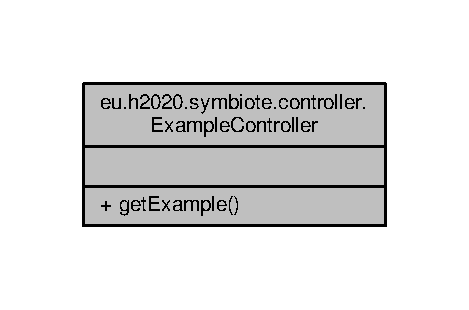
\includegraphics[width=225pt]{classeu_1_1h2020_1_1symbiote_1_1controller_1_1ExampleController__coll__graph}
\end{center}
\end{figure}
\subsection*{Public Member Functions}
\begin{DoxyCompactItemize}
\item 
\mbox{\Hypertarget{classeu_1_1h2020_1_1symbiote_1_1controller_1_1ExampleController_a08f9ba931b4a8f0a69a80d5785c0f414}\label{classeu_1_1h2020_1_1symbiote_1_1controller_1_1ExampleController_a08f9ba931b4a8f0a69a80d5785c0f414}} 
Deferred\+Result$<$ Response\+Entity$<$?$>$ $>$ {\bfseries get\+Example} (@Path\+Variable String value)  throws Exception 
\end{DoxyCompactItemize}


The documentation for this class was generated from the following file\+:\begin{DoxyCompactItemize}
\item 
src/main/java/eu/h2020/symbiote/controller/Example\+Controller.\+java\end{DoxyCompactItemize}

\hypertarget{classeu_1_1h2020_1_1symbiote_1_1InterworkingInterfaceApplication}{}\section{eu.\+h2020.\+symbiote.\+Interworking\+Interface\+Application Class Reference}
\label{classeu_1_1h2020_1_1symbiote_1_1InterworkingInterfaceApplication}\index{eu.\+h2020.\+symbiote.\+Interworking\+Interface\+Application@{eu.\+h2020.\+symbiote.\+Interworking\+Interface\+Application}}


Inheritance diagram for eu.\+h2020.\+symbiote.\+Interworking\+Interface\+Application\+:\nopagebreak
\begin{figure}[H]
\begin{center}
\leavevmode
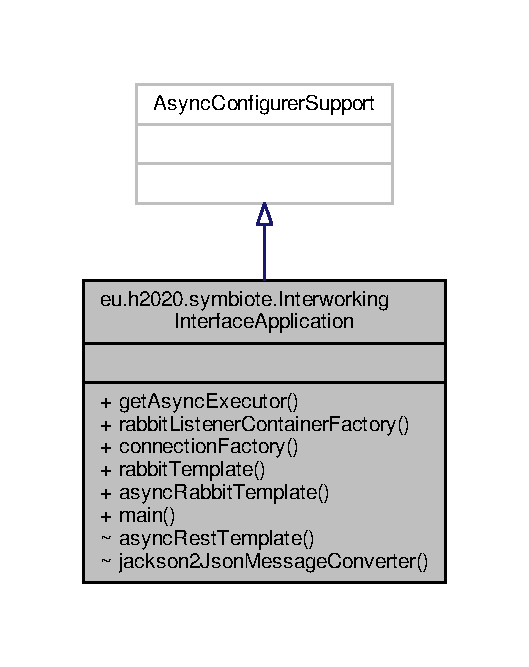
\includegraphics[width=254pt]{classeu_1_1h2020_1_1symbiote_1_1InterworkingInterfaceApplication__inherit__graph}
\end{center}
\end{figure}


Collaboration diagram for eu.\+h2020.\+symbiote.\+Interworking\+Interface\+Application\+:\nopagebreak
\begin{figure}[H]
\begin{center}
\leavevmode
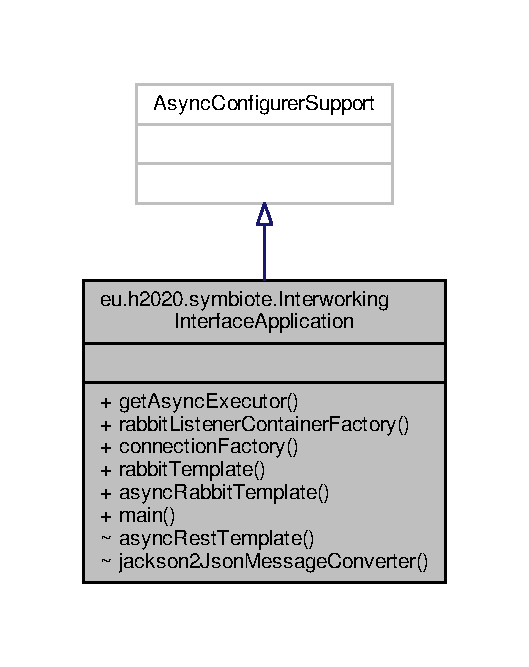
\includegraphics[width=254pt]{classeu_1_1h2020_1_1symbiote_1_1InterworkingInterfaceApplication__coll__graph}
\end{center}
\end{figure}
\subsection*{Public Member Functions}
\begin{DoxyCompactItemize}
\item 
\mbox{\Hypertarget{classeu_1_1h2020_1_1symbiote_1_1InterworkingInterfaceApplication_af4632289d17d2ab6eab0d66dc49a4fe5}\label{classeu_1_1h2020_1_1symbiote_1_1InterworkingInterfaceApplication_af4632289d17d2ab6eab0d66dc49a4fe5}} 
Executor {\bfseries get\+Async\+Executor} ()
\item 
\mbox{\Hypertarget{classeu_1_1h2020_1_1symbiote_1_1InterworkingInterfaceApplication_a17abcc8766dfac302cda76de4fc239fc}\label{classeu_1_1h2020_1_1symbiote_1_1InterworkingInterfaceApplication_a17abcc8766dfac302cda76de4fc239fc}} 
Simple\+Rabbit\+Listener\+Container\+Factory {\bfseries rabbit\+Listener\+Container\+Factory} (Connection\+Factory connection\+Factory)
\item 
\mbox{\Hypertarget{classeu_1_1h2020_1_1symbiote_1_1InterworkingInterfaceApplication_a6846e372032cd37bb5b3a187c8c8c70c}\label{classeu_1_1h2020_1_1symbiote_1_1InterworkingInterfaceApplication_a6846e372032cd37bb5b3a187c8c8c70c}} 
Connection\+Factory {\bfseries connection\+Factory} ()  throws Exception 
\item 
\mbox{\Hypertarget{classeu_1_1h2020_1_1symbiote_1_1InterworkingInterfaceApplication_ad8d56234a0dc97acb64e41eaf4b22691}\label{classeu_1_1h2020_1_1symbiote_1_1InterworkingInterfaceApplication_ad8d56234a0dc97acb64e41eaf4b22691}} 
Rabbit\+Template {\bfseries rabbit\+Template} (Connection\+Factory connection\+Factory, Jackson2\+Json\+Message\+Converter jackson2\+Json\+Message\+Converter)
\item 
Async\+Rabbit\+Template \hyperlink{classeu_1_1h2020_1_1symbiote_1_1InterworkingInterfaceApplication_a45f372aa4f5e90820f58913d5c2377c5}{async\+Rabbit\+Template} (Rabbit\+Template rabbit\+Template)
\end{DoxyCompactItemize}
\subsection*{Static Public Member Functions}
\begin{DoxyCompactItemize}
\item 
\mbox{\Hypertarget{classeu_1_1h2020_1_1symbiote_1_1InterworkingInterfaceApplication_a2a665798ab250c514ac683becc6216e1}\label{classeu_1_1h2020_1_1symbiote_1_1InterworkingInterfaceApplication_a2a665798ab250c514ac683becc6216e1}} 
static void {\bfseries main} (String\mbox{[}$\,$\mbox{]} args)
\end{DoxyCompactItemize}


\subsection{Detailed Description}
Created by mateuszl on 22.\+09.\+2016. 

\subsection{Member Function Documentation}
\mbox{\Hypertarget{classeu_1_1h2020_1_1symbiote_1_1InterworkingInterfaceApplication_a45f372aa4f5e90820f58913d5c2377c5}\label{classeu_1_1h2020_1_1symbiote_1_1InterworkingInterfaceApplication_a45f372aa4f5e90820f58913d5c2377c5}} 
\index{eu\+::h2020\+::symbiote\+::\+Interworking\+Interface\+Application@{eu\+::h2020\+::symbiote\+::\+Interworking\+Interface\+Application}!async\+Rabbit\+Template@{async\+Rabbit\+Template}}
\index{async\+Rabbit\+Template@{async\+Rabbit\+Template}!eu\+::h2020\+::symbiote\+::\+Interworking\+Interface\+Application@{eu\+::h2020\+::symbiote\+::\+Interworking\+Interface\+Application}}
\subsubsection{\texorpdfstring{async\+Rabbit\+Template()}{asyncRabbitTemplate()}}
{\footnotesize\ttfamily Async\+Rabbit\+Template eu.\+h2020.\+symbiote.\+Interworking\+Interface\+Application.\+async\+Rabbit\+Template (\begin{DoxyParamCaption}\item[{Rabbit\+Template}]{rabbit\+Template }\end{DoxyParamCaption})}

The following Async\+Rabbit\+Template constructor uses \char`\"{}\+Direct reply\+To\char`\"{} for replies.

The documentation for this class was generated from the following file\+:\begin{DoxyCompactItemize}
\item 
src/main/java/eu/h2020/symbiote/Interworking\+Interface\+Application.\+java\end{DoxyCompactItemize}

\hypertarget{classeu_1_1h2020_1_1symbiote_1_1controller_1_1InterworkingInterfaceController}{}\section{eu.\+h2020.\+symbiote.\+controller.\+Interworking\+Interface\+Controller Class Reference}
\label{classeu_1_1h2020_1_1symbiote_1_1controller_1_1InterworkingInterfaceController}\index{eu.\+h2020.\+symbiote.\+controller.\+Interworking\+Interface\+Controller@{eu.\+h2020.\+symbiote.\+controller.\+Interworking\+Interface\+Controller}}


Collaboration diagram for eu.\+h2020.\+symbiote.\+controller.\+Interworking\+Interface\+Controller\+:\nopagebreak
\begin{figure}[H]
\begin{center}
\leavevmode
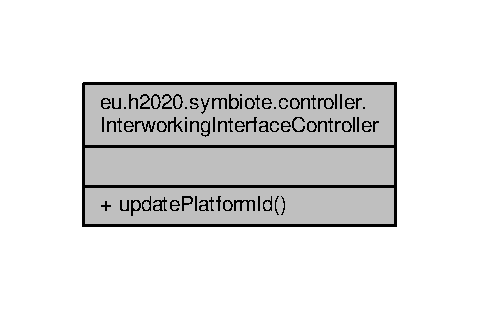
\includegraphics[width=230pt]{classeu_1_1h2020_1_1symbiote_1_1controller_1_1InterworkingInterfaceController__coll__graph}
\end{center}
\end{figure}
\subsection*{Public Member Functions}
\begin{DoxyCompactItemize}
\item 
Response\+Entity$<$ String $>$ \hyperlink{classeu_1_1h2020_1_1symbiote_1_1controller_1_1InterworkingInterfaceController_a6ff9bf0ef30e7e2a34b2d89e77399a59}{update\+Platform\+Id} (@Path\+Variable String id)  throws Exception 
\end{DoxyCompactItemize}


\subsection{Detailed Description}
\subsection*{General Rest\+Controller for Interworking Interface}

\begin{DoxyAuthor}{Author}
Vasileios Glykantzis 
\end{DoxyAuthor}
\begin{DoxyVersion}{Version}
1.\+0 
\end{DoxyVersion}
\begin{DoxySince}{Since}
2017-\/01-\/26 
\end{DoxySince}


\subsection{Member Function Documentation}
\mbox{\Hypertarget{classeu_1_1h2020_1_1symbiote_1_1controller_1_1InterworkingInterfaceController_a6ff9bf0ef30e7e2a34b2d89e77399a59}\label{classeu_1_1h2020_1_1symbiote_1_1controller_1_1InterworkingInterfaceController_a6ff9bf0ef30e7e2a34b2d89e77399a59}} 
\index{eu\+::h2020\+::symbiote\+::controller\+::\+Interworking\+Interface\+Controller@{eu\+::h2020\+::symbiote\+::controller\+::\+Interworking\+Interface\+Controller}!update\+Platform\+Id@{update\+Platform\+Id}}
\index{update\+Platform\+Id@{update\+Platform\+Id}!eu\+::h2020\+::symbiote\+::controller\+::\+Interworking\+Interface\+Controller@{eu\+::h2020\+::symbiote\+::controller\+::\+Interworking\+Interface\+Controller}}
\subsubsection{\texorpdfstring{update\+Platform\+Id()}{updatePlatformId()}}
{\footnotesize\ttfamily Response\+Entity$<$String$>$ eu.\+h2020.\+symbiote.\+controller.\+Interworking\+Interface\+Controller.\+update\+Platform\+Id (\begin{DoxyParamCaption}\item[{@Path\+Variable String}]{id }\end{DoxyParamCaption}) throws Exception}

Update the platform id with a G\+ET request. This interface listens to G\+ET requests for updating the platform id at runtime and notifies the platform-\/side components.


\begin{DoxyParams}{Parameters}
{\em id} & The new platform id \\
\hline
\end{DoxyParams}


The documentation for this class was generated from the following file\+:\begin{DoxyCompactItemize}
\item 
src/main/java/eu/h2020/symbiote/controller/Interworking\+Interface\+Controller.\+java\end{DoxyCompactItemize}

\hypertarget{classeu_1_1h2020_1_1symbiote_1_1controller_1_1RabbitMQCallback}{}\section{eu.\+h2020.\+symbiote.\+controller.\+Rabbit\+M\+Q\+Callback$<$ T $>$ Class Template Reference}
\label{classeu_1_1h2020_1_1symbiote_1_1controller_1_1RabbitMQCallback}\index{eu.\+h2020.\+symbiote.\+controller.\+Rabbit\+M\+Q\+Callback$<$ T $>$@{eu.\+h2020.\+symbiote.\+controller.\+Rabbit\+M\+Q\+Callback$<$ T $>$}}


Inheritance diagram for eu.\+h2020.\+symbiote.\+controller.\+Rabbit\+M\+Q\+Callback$<$ T $>$\+:
\nopagebreak
\begin{figure}[H]
\begin{center}
\leavevmode
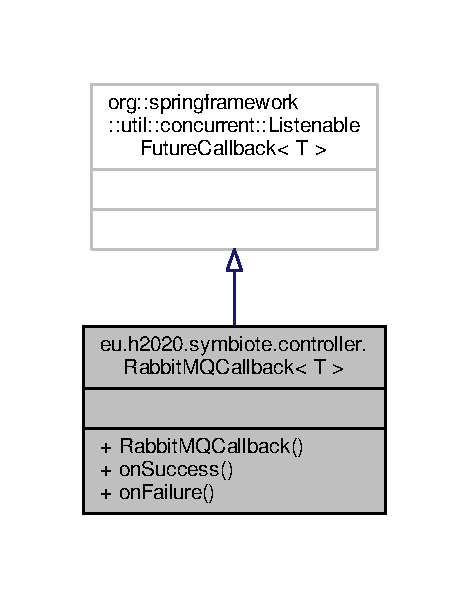
\includegraphics[width=225pt]{classeu_1_1h2020_1_1symbiote_1_1controller_1_1RabbitMQCallback__inherit__graph}
\end{center}
\end{figure}


Collaboration diagram for eu.\+h2020.\+symbiote.\+controller.\+Rabbit\+M\+Q\+Callback$<$ T $>$\+:
\nopagebreak
\begin{figure}[H]
\begin{center}
\leavevmode
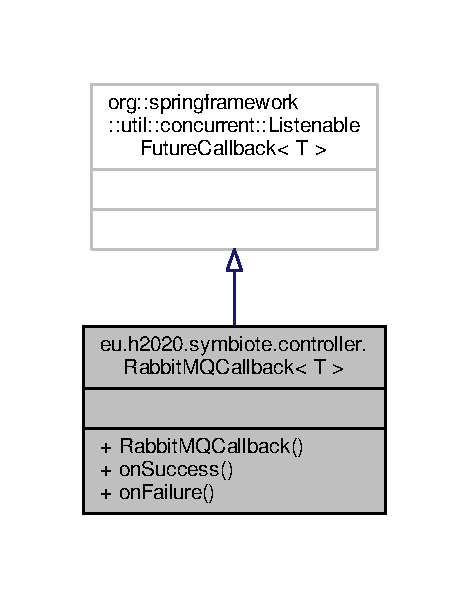
\includegraphics[width=225pt]{classeu_1_1h2020_1_1symbiote_1_1controller_1_1RabbitMQCallback__coll__graph}
\end{center}
\end{figure}
\subsection*{Public Member Functions}
\begin{DoxyCompactItemize}
\item 
\hyperlink{classeu_1_1h2020_1_1symbiote_1_1controller_1_1RabbitMQCallback_af36ac8a5a331017d599f76c768a7bdab}{Rabbit\+M\+Q\+Callback} (String request, Deferred\+Result deferred\+Result)
\item 
\mbox{\Hypertarget{classeu_1_1h2020_1_1symbiote_1_1controller_1_1RabbitMQCallback_a8a046df4e56ad0350dda9de300c6e090}\label{classeu_1_1h2020_1_1symbiote_1_1controller_1_1RabbitMQCallback_a8a046df4e56ad0350dda9de300c6e090}} 
void {\bfseries on\+Success} (T result)
\item 
\mbox{\Hypertarget{classeu_1_1h2020_1_1symbiote_1_1controller_1_1RabbitMQCallback_ac2d139f5ae551eb2b87aef0b022cd1d6}\label{classeu_1_1h2020_1_1symbiote_1_1controller_1_1RabbitMQCallback_ac2d139f5ae551eb2b87aef0b022cd1d6}} 
void {\bfseries on\+Failure} (Throwable ex)
\end{DoxyCompactItemize}


\subsection{Detailed Description}
\subsection*{A Callback for listening to asynchronous Rabbit\+MQ replies}

This class extends the Listenable\+Future\+Callback class and uses the Deferred\+Result class for replying asynchronously to the H\+T\+TP Request received by a controller with the Spring A\+M\+QP reply it receives.

\begin{DoxyAuthor}{Author}
Vasileios Glykantzis 
\end{DoxyAuthor}
\begin{DoxyVersion}{Version}
1.\+0 
\end{DoxyVersion}
\begin{DoxySince}{Since}
2017-\/01-\/26 
\end{DoxySince}


\subsection{Constructor \& Destructor Documentation}
\mbox{\Hypertarget{classeu_1_1h2020_1_1symbiote_1_1controller_1_1RabbitMQCallback_af36ac8a5a331017d599f76c768a7bdab}\label{classeu_1_1h2020_1_1symbiote_1_1controller_1_1RabbitMQCallback_af36ac8a5a331017d599f76c768a7bdab}} 
\index{eu\+::h2020\+::symbiote\+::controller\+::\+Rabbit\+M\+Q\+Callback@{eu\+::h2020\+::symbiote\+::controller\+::\+Rabbit\+M\+Q\+Callback}!Rabbit\+M\+Q\+Callback@{Rabbit\+M\+Q\+Callback}}
\index{Rabbit\+M\+Q\+Callback@{Rabbit\+M\+Q\+Callback}!eu\+::h2020\+::symbiote\+::controller\+::\+Rabbit\+M\+Q\+Callback@{eu\+::h2020\+::symbiote\+::controller\+::\+Rabbit\+M\+Q\+Callback}}
\subsubsection{\texorpdfstring{Rabbit\+M\+Q\+Callback()}{RabbitMQCallback()}}
{\footnotesize\ttfamily \hyperlink{classeu_1_1h2020_1_1symbiote_1_1controller_1_1RabbitMQCallback}{eu.\+h2020.\+symbiote.\+controller.\+Rabbit\+M\+Q\+Callback}$<$ T $>$.\hyperlink{classeu_1_1h2020_1_1symbiote_1_1controller_1_1RabbitMQCallback}{Rabbit\+M\+Q\+Callback} (\begin{DoxyParamCaption}\item[{String}]{request,  }\item[{Deferred\+Result}]{deferred\+Result }\end{DoxyParamCaption})}

Constructor of the \hyperlink{classeu_1_1h2020_1_1symbiote_1_1controller_1_1RabbitMQCallback}{Rabbit\+M\+Q\+Callback}


\begin{DoxyParams}{Parameters}
{\em request} & String describing the type of request. Used in logging. \\
\hline
{\em deferred\+Result} & The deferred\+Result which is modified to serve the H\+T\+TP request. \\
\hline
\end{DoxyParams}


The documentation for this class was generated from the following file\+:\begin{DoxyCompactItemize}
\item 
src/main/java/eu/h2020/symbiote/controller/Rabbit\+M\+Q\+Callback.\+java\end{DoxyCompactItemize}

\hypertarget{classeu_1_1h2020_1_1symbiote_1_1controller_1_1RapRestController}{}\section{eu.\+h2020.\+symbiote.\+controller.\+Rap\+Rest\+Controller Class Reference}
\label{classeu_1_1h2020_1_1symbiote_1_1controller_1_1RapRestController}\index{eu.\+h2020.\+symbiote.\+controller.\+Rap\+Rest\+Controller@{eu.\+h2020.\+symbiote.\+controller.\+Rap\+Rest\+Controller}}


Collaboration diagram for eu.\+h2020.\+symbiote.\+controller.\+Rap\+Rest\+Controller\+:
\nopagebreak
\begin{figure}[H]
\begin{center}
\leavevmode
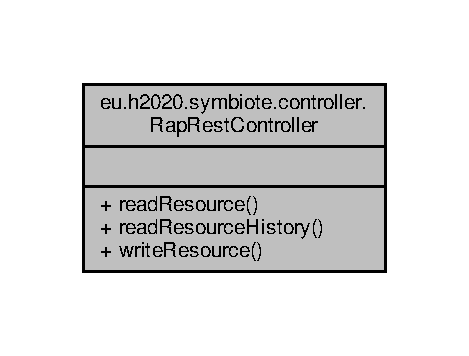
\includegraphics[width=225pt]{classeu_1_1h2020_1_1symbiote_1_1controller_1_1RapRestController__coll__graph}
\end{center}
\end{figure}
\subsection*{Public Member Functions}
\begin{DoxyCompactItemize}
\item 
Deferred\+Result$<$ Response\+Entity$<$?$>$ $>$ \hyperlink{classeu_1_1h2020_1_1symbiote_1_1controller_1_1RapRestController_a02b5cac53d1bb33fb9e89cfc705511f4}{read\+Resource} (@Path\+Variable String resource\+Id)  throws Exception 
\item 
Deferred\+Result$<$ Response\+Entity$<$?$>$ $>$ \hyperlink{classeu_1_1h2020_1_1symbiote_1_1controller_1_1RapRestController_a11fc8b8068e57e32a81b1d3c835cded4}{read\+Resource\+History} (@Path\+Variable String resource\+Id)  throws Exception 
\item 
Deferred\+Result$<$ Response\+Entity$<$?$>$ $>$ \hyperlink{classeu_1_1h2020_1_1symbiote_1_1controller_1_1RapRestController_a2880be887baef0ec6a60627f7c9dc927}{write\+Resource} (@Path\+Variable String resource\+Id, @Request\+Body String value)  throws Exception 
\end{DoxyCompactItemize}


\subsection{Detailed Description}
\subsection*{Rest\+Controller for Resource Access Proxy component}

This class exposes R\+E\+ST interfaces for allowing access to the Resource Access Proxy component from the external world (e.\+g. applications, enablers or the symb\+Io\+Te Core.)

\begin{DoxyAuthor}{Author}
Vasileios Glykantzis 
\end{DoxyAuthor}
\begin{DoxyVersion}{Version}
1.\+0 
\end{DoxyVersion}
\begin{DoxySince}{Since}
2017-\/01-\/26 
\end{DoxySince}


\subsection{Member Function Documentation}
\mbox{\Hypertarget{classeu_1_1h2020_1_1symbiote_1_1controller_1_1RapRestController_a02b5cac53d1bb33fb9e89cfc705511f4}\label{classeu_1_1h2020_1_1symbiote_1_1controller_1_1RapRestController_a02b5cac53d1bb33fb9e89cfc705511f4}} 
\index{eu\+::h2020\+::symbiote\+::controller\+::\+Rap\+Rest\+Controller@{eu\+::h2020\+::symbiote\+::controller\+::\+Rap\+Rest\+Controller}!read\+Resource@{read\+Resource}}
\index{read\+Resource@{read\+Resource}!eu\+::h2020\+::symbiote\+::controller\+::\+Rap\+Rest\+Controller@{eu\+::h2020\+::symbiote\+::controller\+::\+Rap\+Rest\+Controller}}
\subsubsection{\texorpdfstring{read\+Resource()}{readResource()}}
{\footnotesize\ttfamily Deferred\+Result$<$Response\+Entity$<$?$>$ $>$ eu.\+h2020.\+symbiote.\+controller.\+Rap\+Rest\+Controller.\+read\+Resource (\begin{DoxyParamCaption}\item[{@Path\+Variable String}]{resource\+Id }\end{DoxyParamCaption}) throws Exception}

R\+E\+ST interface for Resource Access Proxy\textquotesingle{}s read\+Resource method. This interface is used to read a value of the resource.


\begin{DoxyParams}{Parameters}
{\em resource\+Id} & The id of the resource to be accessed \\
\hline
\end{DoxyParams}

\begin{DoxyExceptions}{Exceptions}
{\em Exception} & \\
\hline
\end{DoxyExceptions}
\mbox{\Hypertarget{classeu_1_1h2020_1_1symbiote_1_1controller_1_1RapRestController_a11fc8b8068e57e32a81b1d3c835cded4}\label{classeu_1_1h2020_1_1symbiote_1_1controller_1_1RapRestController_a11fc8b8068e57e32a81b1d3c835cded4}} 
\index{eu\+::h2020\+::symbiote\+::controller\+::\+Rap\+Rest\+Controller@{eu\+::h2020\+::symbiote\+::controller\+::\+Rap\+Rest\+Controller}!read\+Resource\+History@{read\+Resource\+History}}
\index{read\+Resource\+History@{read\+Resource\+History}!eu\+::h2020\+::symbiote\+::controller\+::\+Rap\+Rest\+Controller@{eu\+::h2020\+::symbiote\+::controller\+::\+Rap\+Rest\+Controller}}
\subsubsection{\texorpdfstring{read\+Resource\+History()}{readResourceHistory()}}
{\footnotesize\ttfamily Deferred\+Result$<$Response\+Entity$<$?$>$ $>$ eu.\+h2020.\+symbiote.\+controller.\+Rap\+Rest\+Controller.\+read\+Resource\+History (\begin{DoxyParamCaption}\item[{@Path\+Variable String}]{resource\+Id }\end{DoxyParamCaption}) throws Exception}

R\+E\+ST interface for Resource Access Proxy\textquotesingle{}s read\+Resource\+History method. This interface is used to read historical values of the resource.


\begin{DoxyParams}{Parameters}
{\em resource\+Id} & The id of the resource to be accessed \\
\hline
\end{DoxyParams}

\begin{DoxyExceptions}{Exceptions}
{\em Exception} & \\
\hline
\end{DoxyExceptions}
\mbox{\Hypertarget{classeu_1_1h2020_1_1symbiote_1_1controller_1_1RapRestController_a2880be887baef0ec6a60627f7c9dc927}\label{classeu_1_1h2020_1_1symbiote_1_1controller_1_1RapRestController_a2880be887baef0ec6a60627f7c9dc927}} 
\index{eu\+::h2020\+::symbiote\+::controller\+::\+Rap\+Rest\+Controller@{eu\+::h2020\+::symbiote\+::controller\+::\+Rap\+Rest\+Controller}!write\+Resource@{write\+Resource}}
\index{write\+Resource@{write\+Resource}!eu\+::h2020\+::symbiote\+::controller\+::\+Rap\+Rest\+Controller@{eu\+::h2020\+::symbiote\+::controller\+::\+Rap\+Rest\+Controller}}
\subsubsection{\texorpdfstring{write\+Resource()}{writeResource()}}
{\footnotesize\ttfamily Deferred\+Result$<$Response\+Entity$<$?$>$ $>$ eu.\+h2020.\+symbiote.\+controller.\+Rap\+Rest\+Controller.\+write\+Resource (\begin{DoxyParamCaption}\item[{@Path\+Variable String}]{resource\+Id,  }\item[{@Request\+Body String}]{value }\end{DoxyParamCaption}) throws Exception}

R\+E\+ST interface for Resource Access Proxy\textquotesingle{}s write\+Resource method. This interface is used to write a value to a resource (i.\+e. actuator)


\begin{DoxyParams}{Parameters}
{\em resource\+Id} & The id of the resource to be accessed \\
\hline
{\em value} & The value to be written to the resource \\
\hline
\end{DoxyParams}

\begin{DoxyExceptions}{Exceptions}
{\em Exception} & \\
\hline
\end{DoxyExceptions}


The documentation for this class was generated from the following file\+:\begin{DoxyCompactItemize}
\item 
src/main/java/eu/h2020/symbiote/controller/Rap\+Rest\+Controller.\+java\end{DoxyCompactItemize}

\hypertarget{classeu_1_1h2020_1_1symbiote_1_1rpcserver_1_1RegistrationHandlerRPCServer}{}\section{eu.\+h2020.\+symbiote.\+rpcserver.\+Registration\+Handler\+R\+P\+C\+Server Class Reference}
\label{classeu_1_1h2020_1_1symbiote_1_1rpcserver_1_1RegistrationHandlerRPCServer}\index{eu.\+h2020.\+symbiote.\+rpcserver.\+Registration\+Handler\+R\+P\+C\+Server@{eu.\+h2020.\+symbiote.\+rpcserver.\+Registration\+Handler\+R\+P\+C\+Server}}


Collaboration diagram for eu.\+h2020.\+symbiote.\+rpcserver.\+Registration\+Handler\+R\+P\+C\+Server\+:\nopagebreak
\begin{figure}[H]
\begin{center}
\leavevmode
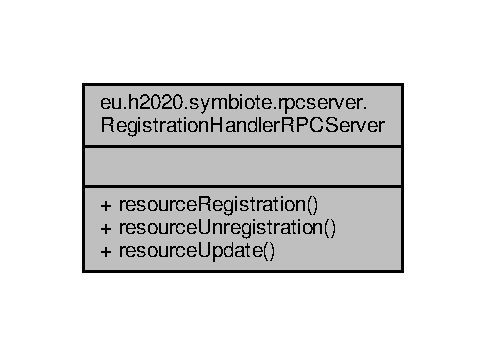
\includegraphics[width=233pt]{classeu_1_1h2020_1_1symbiote_1_1rpcserver_1_1RegistrationHandlerRPCServer__coll__graph}
\end{center}
\end{figure}
\subsection*{Public Member Functions}
\begin{DoxyCompactItemize}
\item 
void \hyperlink{classeu_1_1h2020_1_1symbiote_1_1rpcserver_1_1RegistrationHandlerRPCServer_a59d3a42c7b9a1b51b7956226abc1d66e}{resource\+Registration} (J\+S\+O\+N\+Object json\+Object, @Headers() Map$<$ String, String $>$ headers)
\item 
void \hyperlink{classeu_1_1h2020_1_1symbiote_1_1rpcserver_1_1RegistrationHandlerRPCServer_acbb159563455460f6a3da99e5353d11a}{resource\+Unregistration} (String id, @Headers() Map$<$ String, String $>$ headers)
\item 
void \hyperlink{classeu_1_1h2020_1_1symbiote_1_1rpcserver_1_1RegistrationHandlerRPCServer_add97d8f15845030d4f09f7db65107bec}{resource\+Update} (J\+S\+O\+N\+Object json\+Object, @Headers() Map$<$ String, String $>$ headers)
\end{DoxyCompactItemize}


\subsection{Detailed Description}
\subsection*{\hyperlink{classeu_1_1h2020_1_1symbiote_1_1rpcserver_1_1RegistrationHandlerRPCServer}{Registration\+Handler\+R\+P\+C\+Server} for Resource Access Proxy component}

This class exposes Spring A\+M\+QP interfaces for allowing Registration Handler to access the external world (e.\+g. applications, enablers or the symb\+Io\+Te Core.)

\begin{DoxyAuthor}{Author}
Vasileios Glykantzis 
\end{DoxyAuthor}
\begin{DoxyVersion}{Version}
1.\+0 
\end{DoxyVersion}
\begin{DoxySince}{Since}
2017-\/01-\/26 
\end{DoxySince}


\subsection{Member Function Documentation}
\mbox{\Hypertarget{classeu_1_1h2020_1_1symbiote_1_1rpcserver_1_1RegistrationHandlerRPCServer_a59d3a42c7b9a1b51b7956226abc1d66e}\label{classeu_1_1h2020_1_1symbiote_1_1rpcserver_1_1RegistrationHandlerRPCServer_a59d3a42c7b9a1b51b7956226abc1d66e}} 
\index{eu\+::h2020\+::symbiote\+::rpcserver\+::\+Registration\+Handler\+R\+P\+C\+Server@{eu\+::h2020\+::symbiote\+::rpcserver\+::\+Registration\+Handler\+R\+P\+C\+Server}!resource\+Registration@{resource\+Registration}}
\index{resource\+Registration@{resource\+Registration}!eu\+::h2020\+::symbiote\+::rpcserver\+::\+Registration\+Handler\+R\+P\+C\+Server@{eu\+::h2020\+::symbiote\+::rpcserver\+::\+Registration\+Handler\+R\+P\+C\+Server}}
\subsubsection{\texorpdfstring{resource\+Registration()}{resourceRegistration()}}
{\footnotesize\ttfamily void eu.\+h2020.\+symbiote.\+rpcserver.\+Registration\+Handler\+R\+P\+C\+Server.\+resource\+Registration (\begin{DoxyParamCaption}\item[{J\+S\+O\+N\+Object}]{json\+Object,  }\item[{@Headers() Map$<$ String, String $>$}]{headers }\end{DoxyParamCaption})}

Spring A\+M\+QP Listener for resource registration requests. This method is invoked when Registration Handler sends a resource registration request and it is responsible for forwarding the message to the symb\+Io\+Te core. As soon as it receives a reply, it manually sends back the response to the Registration Handler via the appropriate message queue by the use of the \hyperlink{classeu_1_1h2020_1_1symbiote_1_1rpcserver_1_1RestAPICallback}{Rest\+A\+P\+I\+Callback}.


\begin{DoxyParams}{Parameters}
{\em json\+Object} & A json\+Object containing the resource description \\
\hline
{\em headers} & The A\+M\+QP headers \\
\hline
\end{DoxyParams}
\mbox{\Hypertarget{classeu_1_1h2020_1_1symbiote_1_1rpcserver_1_1RegistrationHandlerRPCServer_acbb159563455460f6a3da99e5353d11a}\label{classeu_1_1h2020_1_1symbiote_1_1rpcserver_1_1RegistrationHandlerRPCServer_acbb159563455460f6a3da99e5353d11a}} 
\index{eu\+::h2020\+::symbiote\+::rpcserver\+::\+Registration\+Handler\+R\+P\+C\+Server@{eu\+::h2020\+::symbiote\+::rpcserver\+::\+Registration\+Handler\+R\+P\+C\+Server}!resource\+Unregistration@{resource\+Unregistration}}
\index{resource\+Unregistration@{resource\+Unregistration}!eu\+::h2020\+::symbiote\+::rpcserver\+::\+Registration\+Handler\+R\+P\+C\+Server@{eu\+::h2020\+::symbiote\+::rpcserver\+::\+Registration\+Handler\+R\+P\+C\+Server}}
\subsubsection{\texorpdfstring{resource\+Unregistration()}{resourceUnregistration()}}
{\footnotesize\ttfamily void eu.\+h2020.\+symbiote.\+rpcserver.\+Registration\+Handler\+R\+P\+C\+Server.\+resource\+Unregistration (\begin{DoxyParamCaption}\item[{String}]{id,  }\item[{@Headers() Map$<$ String, String $>$}]{headers }\end{DoxyParamCaption})}

Spring A\+M\+QP Listener for resource unregistration requests. This method is invoked when Registration Handler sends a resource registration request and it is responsible for forwarding the message to the symb\+Io\+Te core. As soon as it receives a reply, it manually sends back the response to the Registration Handler via the appropriate message queue by the use of the \hyperlink{classeu_1_1h2020_1_1symbiote_1_1rpcserver_1_1RestAPICallback}{Rest\+A\+P\+I\+Callback}.


\begin{DoxyParams}{Parameters}
{\em id} & The id of the resource to be deleted \\
\hline
{\em headers} & The A\+M\+QP headers \\
\hline
\end{DoxyParams}
\mbox{\Hypertarget{classeu_1_1h2020_1_1symbiote_1_1rpcserver_1_1RegistrationHandlerRPCServer_add97d8f15845030d4f09f7db65107bec}\label{classeu_1_1h2020_1_1symbiote_1_1rpcserver_1_1RegistrationHandlerRPCServer_add97d8f15845030d4f09f7db65107bec}} 
\index{eu\+::h2020\+::symbiote\+::rpcserver\+::\+Registration\+Handler\+R\+P\+C\+Server@{eu\+::h2020\+::symbiote\+::rpcserver\+::\+Registration\+Handler\+R\+P\+C\+Server}!resource\+Update@{resource\+Update}}
\index{resource\+Update@{resource\+Update}!eu\+::h2020\+::symbiote\+::rpcserver\+::\+Registration\+Handler\+R\+P\+C\+Server@{eu\+::h2020\+::symbiote\+::rpcserver\+::\+Registration\+Handler\+R\+P\+C\+Server}}
\subsubsection{\texorpdfstring{resource\+Update()}{resourceUpdate()}}
{\footnotesize\ttfamily void eu.\+h2020.\+symbiote.\+rpcserver.\+Registration\+Handler\+R\+P\+C\+Server.\+resource\+Update (\begin{DoxyParamCaption}\item[{J\+S\+O\+N\+Object}]{json\+Object,  }\item[{@Headers() Map$<$ String, String $>$}]{headers }\end{DoxyParamCaption})}

Spring A\+M\+QP Listener for resource update requests. This method is invoked when Registration Handler sends a resource registration request and it is responsible for forwarding the message to the symb\+Io\+Te core. As soon as it receives a reply, it manually sends back the response to the Registration Handler via the appropriate message queue by the use of the \hyperlink{classeu_1_1h2020_1_1symbiote_1_1rpcserver_1_1RestAPICallback}{Rest\+A\+P\+I\+Callback}.


\begin{DoxyParams}{Parameters}
{\em json\+Object} & A json\+Object containing the resource description \\
\hline
{\em headers} & The A\+M\+QP headers \\
\hline
\end{DoxyParams}


The documentation for this class was generated from the following file\+:\begin{DoxyCompactItemize}
\item 
src/main/java/eu/h2020/symbiote/rpcserver/Registration\+Handler\+R\+P\+C\+Server.\+java\end{DoxyCompactItemize}

\hypertarget{classeu_1_1h2020_1_1symbiote_1_1rpcserver_1_1RestAPICallback}{}\section{eu.\+h2020.\+symbiote.\+rpcserver.\+Rest\+A\+P\+I\+Callback$<$ T $>$ Class Template Reference}
\label{classeu_1_1h2020_1_1symbiote_1_1rpcserver_1_1RestAPICallback}\index{eu.\+h2020.\+symbiote.\+rpcserver.\+Rest\+A\+P\+I\+Callback$<$ T $>$@{eu.\+h2020.\+symbiote.\+rpcserver.\+Rest\+A\+P\+I\+Callback$<$ T $>$}}


Inheritance diagram for eu.\+h2020.\+symbiote.\+rpcserver.\+Rest\+A\+P\+I\+Callback$<$ T $>$\+:\nopagebreak
\begin{figure}[H]
\begin{center}
\leavevmode
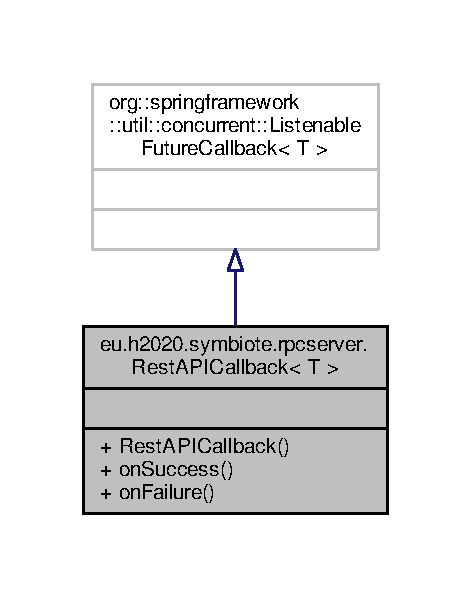
\includegraphics[width=226pt]{classeu_1_1h2020_1_1symbiote_1_1rpcserver_1_1RestAPICallback__inherit__graph}
\end{center}
\end{figure}


Collaboration diagram for eu.\+h2020.\+symbiote.\+rpcserver.\+Rest\+A\+P\+I\+Callback$<$ T $>$\+:\nopagebreak
\begin{figure}[H]
\begin{center}
\leavevmode
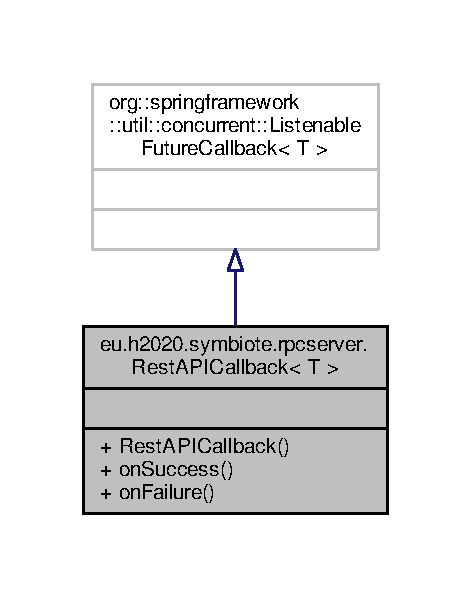
\includegraphics[width=226pt]{classeu_1_1h2020_1_1symbiote_1_1rpcserver_1_1RestAPICallback__coll__graph}
\end{center}
\end{figure}
\subsection*{Public Member Functions}
\begin{DoxyCompactItemize}
\item 
\hyperlink{classeu_1_1h2020_1_1symbiote_1_1rpcserver_1_1RestAPICallback_ad5c5d0f8a589e0555039a1742642789a}{Rest\+A\+P\+I\+Callback} (String request, Map$<$ String, String $>$ headers, Queue$<$ Listenable\+Future$<$ Response\+Entity$<$ J\+S\+O\+N\+Object $>$$>$$>$ futures\+Queue, Listenable\+Future$<$ Response\+Entity$<$ J\+S\+O\+N\+Object $>$$>$ future, Rabbit\+Template rabbit\+Template)
\item 
\mbox{\Hypertarget{classeu_1_1h2020_1_1symbiote_1_1rpcserver_1_1RestAPICallback_a7b1388238a670c0a6be303cc827c956b}\label{classeu_1_1h2020_1_1symbiote_1_1rpcserver_1_1RestAPICallback_a7b1388238a670c0a6be303cc827c956b}} 
void {\bfseries on\+Success} (T result)
\item 
\mbox{\Hypertarget{classeu_1_1h2020_1_1symbiote_1_1rpcserver_1_1RestAPICallback_a0dd62fd546fc035c1cb3324194812710}\label{classeu_1_1h2020_1_1symbiote_1_1rpcserver_1_1RestAPICallback_a0dd62fd546fc035c1cb3324194812710}} 
void {\bfseries on\+Failure} (Throwable t)
\end{DoxyCompactItemize}


\subsection{Detailed Description}
\subsection*{A Callback for listening to asynchronous R\+E\+ST replies }

This class extends the Listenable\+Future\+Callback class and manually sends back the H\+T\+TP reply it receives to the specified \char`\"{}reply-\/\+To\char`\"{} queue of the Rabbit\+MQ request received by the R\+P\+C\+Server.

\begin{DoxyAuthor}{Author}
Vasileios Glykantzis 
\end{DoxyAuthor}
\begin{DoxyVersion}{Version}
1.\+0 
\end{DoxyVersion}
\begin{DoxySince}{Since}
2017-\/01-\/26 
\end{DoxySince}


\subsection{Constructor \& Destructor Documentation}
\mbox{\Hypertarget{classeu_1_1h2020_1_1symbiote_1_1rpcserver_1_1RestAPICallback_ad5c5d0f8a589e0555039a1742642789a}\label{classeu_1_1h2020_1_1symbiote_1_1rpcserver_1_1RestAPICallback_ad5c5d0f8a589e0555039a1742642789a}} 
\index{eu\+::h2020\+::symbiote\+::rpcserver\+::\+Rest\+A\+P\+I\+Callback@{eu\+::h2020\+::symbiote\+::rpcserver\+::\+Rest\+A\+P\+I\+Callback}!Rest\+A\+P\+I\+Callback@{Rest\+A\+P\+I\+Callback}}
\index{Rest\+A\+P\+I\+Callback@{Rest\+A\+P\+I\+Callback}!eu\+::h2020\+::symbiote\+::rpcserver\+::\+Rest\+A\+P\+I\+Callback@{eu\+::h2020\+::symbiote\+::rpcserver\+::\+Rest\+A\+P\+I\+Callback}}
\subsubsection{\texorpdfstring{Rest\+A\+P\+I\+Callback()}{RestAPICallback()}}
{\footnotesize\ttfamily \hyperlink{classeu_1_1h2020_1_1symbiote_1_1rpcserver_1_1RestAPICallback}{eu.\+h2020.\+symbiote.\+rpcserver.\+Rest\+A\+P\+I\+Callback}$<$ T $>$.\hyperlink{classeu_1_1h2020_1_1symbiote_1_1rpcserver_1_1RestAPICallback}{Rest\+A\+P\+I\+Callback} (\begin{DoxyParamCaption}\item[{String}]{request,  }\item[{Map$<$ String, String $>$}]{headers,  }\item[{Queue$<$ Listenable\+Future$<$ Response\+Entity$<$ J\+S\+O\+N\+Object $>$$>$$>$}]{futures\+Queue,  }\item[{Listenable\+Future$<$ Response\+Entity$<$ J\+S\+O\+N\+Object $>$$>$}]{future,  }\item[{Rabbit\+Template}]{rabbit\+Template }\end{DoxyParamCaption})}

Constructor of the \hyperlink{classeu_1_1h2020_1_1symbiote_1_1rpcserver_1_1RestAPICallback}{Rest\+A\+P\+I\+Callback}


\begin{DoxyParams}{Parameters}
{\em request} & String describing the type of request. Used in logging. \\
\hline
{\em headers} & The headers of the A\+M\+QP request \\
\hline
{\em futures\+Queue} & The Queue containing all the not yet served Listenable\+Futures \\
\hline
{\em future} & The Listenable\+Future which the class is set as callback for. \\
\hline
{\em rabbit\+Template} & The Rabbit\+Template used to send the Spring A\+M\+QP reply \\
\hline
\end{DoxyParams}


The documentation for this class was generated from the following file\+:\begin{DoxyCompactItemize}
\item 
src/main/java/eu/h2020/symbiote/rpcserver/Rest\+A\+P\+I\+Callback.\+java\end{DoxyCompactItemize}

%--- End generated contents ---

% Index
\backmatter
\newpage
\phantomsection
\clearemptydoublepage
\addcontentsline{toc}{chapter}{Index}
\printindex

\end{document}
